\documentclass{article} 
\usepackage{graphicx}
\usepackage{animate}
\usepackage{multicol}
\usepackage{hyperref}
\usepackage{amsmath}

\usepackage[utf8]{inputenc}
\usepackage[style=alphabetic]{biblatex}
\addbibresource{references.bib}

\begin{document}

\begin{titlepage}
    \begin{center}
        \vspace*{1cm}
        
        \Large
        \textbf{Particle swarm optimization to the MLJ machine learning toolbox}
        
        \vspace{0.25cm}
        
        \text{Google Summer of Code 2021 Proposal}
        \vspace{0.5cm}
        
        
        \vspace{1.5cm}
        
        \Large
        \textbf{Quazi Irfan\\}
        \text{Mentors: Anthony Blaom, Sebastian Vollmer}
        
        \vspace{0.5cm}
        \animategraphics[loop,autoplay, width=0.65\linewidth]{1}{./plots/cover/plot}{1}{25}
        \vspace{0.5cm}
        
        \small
        \begin{multicols}{2}
        \begin{flushleft}
        \textbf{MS Student in Statistics} \\
        South Dakota State University
        
        Contact: 704 12th Ave, Apt 3 \\
        Brookings, South Dakota, 57006 \\
        
        Email: quazirfan@gmail.com; quazi.irfan@jacks.sdstate.edu\\
        Websites: github.com/quazi-irfan/ \\
        Slack nick: Quazi Irfan \\
        Telephone number: +1 386 334 4792
        \end{flushleft}
        
        \vspace{0.8cm}
        
        \columnbreak
        \begin{flushleft}
        \textbf{Google Summer of Code '21} \\
        Organization: Julia Language \\
        Package: MLJ / MLJ Tuning 
        \end{flushleft}
        \end{multicols}
        \footnote{Please use Adobe Acrobat Reader to open this PDF as all plots are animated.}
        \footnote{No code is included in this PDF. All code are hosted at \href{https://github.com/quazi-irfan/Julia_PSO_GSoC21}{my Github repo}}
    \end{center}
\end{titlepage}
\pagebreak

\tableofcontents
\pagebreak

\section{Introduction}

MLJ(Machine Learning in Julia) is a toolbox written in Julia that provided uniform interface for fitting, evaluating, tuning and benchmark models. This toolbox uses scientific types to ease handling different data type and allows model composition using pipelining.

Each MLJ model can be tuned with a set of parameters known hyperparameters. Choosing the correct hyperparameter value is critical for optimal model performance. Currently, MLJ provides a satellite package called MLJ-Tuning for automate the hyperparameter tuning process. But the number of optimization algorithms available at MLJ-Tuning is limited. This goal of this proposal is to add Particle Swarm optimization as a new optimization algorithm.

Particle swarm optimization(PSO) is easy to understand optimization algorithm with highly active research community. In this proposal, I'll talk about the simple particle swarm optimization implementation that can handle single variable periodic function. I'll also talk about the possible PSO variants and show examples in Python, R and Julia. Finally I'll mention how PSO can be incorporated into MLJ.

\section{Particle Swarm Optimization}

Particle Swarm Optimization is a nature inspired numerical optimization method to minimize a function by generating and manipulating a swarm of particle(that represents possible solutions) and improve those solutions iteratively by simulating the behaviour of a bird flocking or a fish schooling.

This algorithm starts with a set of candidate solution that are distributed over the space that is assumed to contain the minimum of the objective function. These candidate solutions are known as particles.

At each step of the algorithm, the particle tries to find a more optimal position for themselves. The position update rules can be expressed as following,

\begin{equation}
x(t+1) = x(t) + v(t+1)
\end{equation}
Where $x(t)$ and $x(t+1)$ are vectors that represents all particle position at time $t$ and $t+1$ and $v(t+1)$ representing the velocity of the particle at time $t+1$

As particles move, it keeps track of its own best position. Each particles also communicate with other particles in the swarm to find best position. At each iteration particle finds its next position using a combination of its personal best from the past and current swarm's best particle position. This loop continues until a stop condition is met.

The velocity update rule for each particle has a stochastic and deterministic part. The deterministic parts are the following,
\begin{enumerate}
\item Inertia component: The velocity of the particle($v(t)$) from last iteration. This serves as a memory of previous movement.
\item Personal component: The distance between the particle's past best position and current position($x_b - x(t)$). This terms makes the particle want to move back to his past best position. 
\item Social component: The distance between the swarm's best position and particle's current position($x_g - x(t)$).  This terms makes the particle want to move towards the swarm's best position.
\end{enumerate}

The personal and social component are multiplied by random values $r_1$ and $r_2$ that follows Uniform[0,1], and these terms introduces stochastic element to each particle movement. They are also multiplied by constant acceleration term $c_1$ and $c_2$.

So, the velocity update equation is the following,

\begin{equation}
v(t+1) = v(t)w + c_1 r_1(t)[x_b - x(t)] +  c_2 r_2(t)[x_g - x(t)]
\end{equation}

In each step of the algorithm, velocity is updated for each particle which is followed by position update. This process continues until a stopping condition is met. In my PSO implementation, I am ruining the algorithm for 25 iterations.

\subsection{Vanilla PSO implementation}

My vanilla PSO implementation can be found here, \cite{irfan_2021VJ}. This implementation can minimizes a function of single variable. I'll demonstrate my PSO implementation by trying to optimize a single variable function, $f(x) = x^2$. Analytically we know that that the function minimizes at 0.

We will generate a swarm of 10 particles from -9 to 9 with interval 2. The graph of $f(x)$ is in blue and the swarm are represented as scatter point in unique colors(Iteration 0). The plot is an animation that will show the updated position of each particle on each iteration, from iteration 1 to 25. In the animated plot, we see a lot of oscillation in the first few iterations and the oscillation slowly dies down after each iteration. Note that the particles are starting to converge after 15 iterations.  

This same observation is also evident in the cost history plot. On the x axis of the cost history graph we have the number of iteration and on y axis we have the cost which is defined as average change in position in two successive iterations. Note that there is a spike in the cost history at the beginning since the initial velocity of the particles are zero and they get too excited by the global minimum resulting in overshooting.

The values of particle position are also present in Table 1. As we can see that the particles are uniformly distribute at Iteration 0, and starts to converge in first few iterations, and by the 10th iteration they are already very close to our analytical solution. By 25th iteration all particles are very close to 0 - which is what we expect.

\begin{center}
\animategraphics[loop,autoplay, width=\linewidth]{1}{./plots/plot}{0}{25}
\end{center}
\begin{center}
\noindent\rule{12cm}{0.1pt}
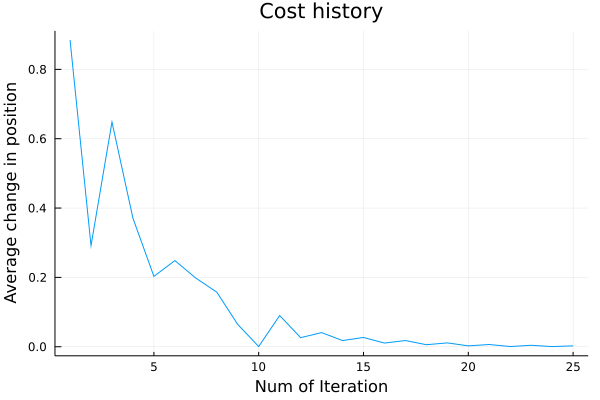
\includegraphics[width=\linewidth]{./plots/CostHistory.png}
\end{center}

\begin{center}
\begin{tabular}{ |c|c|c|c|c|c|c|c|c| } 

\hline
Init(0) & 1 & 2 & ... & 5 & ... & 10 & ... & 25\\
\hline
-8.32 &  0.60 &  0.60 & ... & -0.25 & ... &  -0.21 & ... & -0.0026\\ 
-6.60 &  0.38 &  0.38 & ... & -0.21 & ... &  -0.16 & ... & -0.0021\\  
-4.68 &  0.13 &  0.13 & ... &  0.13 & ... &  -0.08 & ... & -0.0012\\  
-2.33 & -0.16 & -0.16 & ... & -0.13 & ... &  -0.07 & ... & -0.0011\\ 
-0.41 & -0.41 &  0.20 & ... &  0.15 & ... &   0.02 & ... & -0.0001\\  
 1.05 & -0.60 & -0.59 & ... & -0.28 & ... &  -0.09 & ... & -0.0018\\ 
 3.26 & -0.88 & -0.88 & ... & -0.50 & ... &  -0.18 & ... & -0.0051\\ 
 5.10 & -1.12 & -1.12 & ... &  0.00 & ... &   0.00 & ... & -0.0001\\  
 7.16 & -1.38 & -1.38 & ... &  0.04 & ... &   0.04 & ... & -0.0005\\ 
 9.47 & -1.68 & -1.68 & ... &  0.08 & ... &   0.08 & ... &  0.0023\\ 
\hline
\end{tabular}
\end{center}

\subsection{Assumptions in vanilla PSO implementation}

I've made the following assumptions in my implementation.
\begin{enumerate}
  \item Particle initialization: 10 particles were generated uniformly in the range $[-9, 9]$, because we know the objective function is minimum at 0. It is important to make sure generated particles cover the area containing the optimal location otherwise it is difficult for PSO to converge. Particle velocity was set to zero. I also had tweak maximum velocity based on the problem.
  \item Swarm connectivity: I am using global best - assuming all particles are connected with other particles in the swarm - similar to a complete graph. Other approaches could involved particles only connected to other particles closer to them based on some measure of distance such as Euclidean distance or spatial similarity.
  \item Control parameters: 
  \subitem Acceleration constant: $c_1$ and $c_2$ are positive acceleration constant that scales the contribution of personal and social component. It was  set to 1.2.
  \subitem Stochastic parameters: $r_1$ and $r_2$ are sampled from Uniform(0,1) in each iteration \cite{engelbrecht2007computational}. These random values introduces the stochastic behaviour to the particles.
  \item Stopping condition: There are many different stopping condition for PSO. I am chosing to stop the algorithm after 25th iteration as it's producing good result. The cost history also shows me that the average change is position is slowing down.
\end{enumerate}

\subsection{Adjusting for periodic function}
As we know period functions are function that satisfied the $f(t + T) = f(t)$. I've updated my implementation that can find the minimum of a  periodic function. I had to make a function that clamps the position of the particle between the period. Here is the algorithm running on sin (left) and cos(right) function. I had to tweak the max velocity clamping to get stable result.

\animategraphics[loop,autoplay, width=0.5\linewidth]{1}{./plots/sin/sin_convergence-}{1}{51}
\animategraphics[loop,autoplay, width=0.5 \linewidth]{1}{./plots/cos/cos-}{1}{26}

\section{PSO Variants - Standard}
The original paper published in 1995 by Kennedy and Eberhart had the following velocity and position update formula for each particle, 
\begin{align*}
v(t+1) &= v(t) + c_1r_1(x_b - x(t)) + c_2r_2(x_g - x(t)) \\
x(t+1) &= x(t) + v(t+1) 
\end{align*}
Where $r_1, r_2$ follows $Uniform(0,1)$. The velocity is clamped between $[-V_{max}, V_{min}]$ to prevent the particles from flying out of the search space \cite{kennedy1995particle}.

PSO is influenced by many parameters such as velocity clamping, particle inertia, dimension of the problem, number of particles, neighbour hood size(global vs local), number of iterations and many other. Some of these variants are described below with example usage in Python, R and Julia.


\subsection{Inertia Weight}
There is no precise method to chose the range of velocity therefore inertia weight($w$) was introduced by \cite{shi1998modified} to replace velocity clamping which modified the velocity update equation to  
\begin{align*} v(t+1) = \boldsymbol{w} v(t) + c_1r_1(x_b - x(t)) + c_2r_2(x_g - x(t))
\end{align*} and it was also found that the algorithm converges if $w > \frac{1}{2}(c_1 + c_2) - 1$ \cite{van2007analysis}. If w \textgreater 1 then velocities increase over time, accelerating towards maximum velocity. If w \textless 1 the particles decelerate until their reach minimum. Large values of w facilitate exploration and small w facilitate local exploration. Weight could also be dynamically by sampling from Gaussian distribution at each iteration and it could also linearly/non-linearly decreasing over time. Alfi and Fateh presented fuzzy PSO where particle dynamically adjust inertia weight according to particle best memories using non-linear model \cite{alfi2011intelligent}. Inertia weight could not completely eliminate the need for velocity clamping.

\subsubsection{Inertia Weight Example in R}
MetaheuristicOpt package in R implements PSO with inertia weight variation. I've ran the optimization function on Rosenbrock $(a =1, b=100)$ and the result of optimization is [0.9996966, 0.9993824] which very close to expected [1,1] \cite{irfan_2021R} Section 1.

\subsection{Velocity}

\subsubsection{Velocity clamping}
As velocity increases in each iteration, it is important to clamp its value to prevent particles from flying out of search space. If $V_{max}$ is too low swarm may be trapped in local minimum. If it's too high then particle may jump over good region. Usually$V_{max}$ are selected to be a fraction of the search space on each dimension. That is,
\begin{align*}
    V_{max} &=  \delta(x_{max} - x_{min})
\end{align*}
The value of $\delta$ is problem dependent, and we can use cross-validation to find the best value \cite{omran2004image}. A problem arises when all velocities are set to $V_{min}$ or $V_{max}$. A solution to this problem is to change $V_max$ over time linearly or exponentially.




\subsubsection{Velocity constriction}
Clerc  proposed the use of constriction factor similar to inertia weight to balance between exploration and exploitation where velocities are constricted by a constant $\chi$ \cite{clerc1999swarm},
\begin{align*}
\chi &= \frac{2k}{|2-\phi - \sqrt{\phi^2 - 4\phi}|} & \text{where } \phi = c_1 r_1 + c_2 r_2 \text{ and } k \in [0,1]
\end{align*}
This updates the velocity update equation to 
\begin{align*}v(t+1) &= \chi[v(t) + c_1r_1(x_b - x(t)) + c_2r_2(x_g - x(t)))]\end{align*}
Here $\phi > 4$  guarantees convergence. It was developed as an alternate to velocity clamping. $\chi$ is evaluated to the range [0,1] which implies the velocity is reduced in each time step. The term $k$ controls the exploration and exploitation ability of the swarm which is set to a constant value. Furthermore, Fan proposed a method where the velocity are multiplied by a scaling factor $(1 - \frac{t}{T})^h$ where t is the number of iteration, T is the maximum number of iteration and h is constant found by trial and error \cite{fan2002modification}.




\subsection{Particle Connectivity}
The performance of PSO strongly depends on how the particles are connected. In a fully connected swarm, each particle can learn about the best particle position in the swarm. Particles are sometimes only connected to its neighbour and the locality of a particle can be calculated using Euclidean distance, spatial similarity, particle index or some other measure. This local variant do not converge as fast but has more exploitative features. Different social structures have been developed for PSO such as star, ring, wheel, pyramid, Von-Neumann and many more. In Von-Neumann social structure particles are connected in a grid, and it has been found to outperform other social networks in large number of problem. It was also found that in fully connected structures perform best for uni-modal problem and less connected structure perform better of multi-modal problem \cite{kennedy1999small}. Ni proposed to use random topology and analyzed its performance. \cite{ni2013new}. Lim proposed PSO with that linearly increasing topology connectivity with time.

Suganthan proposed particle neighbour that grows with iteration \cite{suganthan1999particle}. The search is initialized with a local best with number of particle in neighbour set to 2, and increases with each iteration until the the neighbour hood contains the entire swarm. 

\subsubsection{Local best Example in Python}
PySwarm implements a local best PSO variant that uses ring topology and locality is defined in terms of distance computed using L2(Euclidean) norm. An example uses the implementation with neighbour size set to 3 and L2 distance set to 2 and trying to minimize the Rosenbrock function with $(a = 1, b = 1)$ and the result of the optimization is 0.99 and 0.99 which very close to what we expect. \cite{irfan_2021P}




\subsection{Particle Number and Initialization}
Large number of particles allows larger parts of search space but increase computation time, and small number of particle lead to insufficient exploration and could result in local optima - therefore 20-100 was accepted according to Bratton \cite{bratton2007defining}. It has also been showed that PSO has the ability to find optimal solution with small swarm size of 10 to 30 paticles \cite{bergh2001effects}. 

Different initialization method has been proposed to ensure the search space is uniformly covered, such as Sobol sequence \cite{parsopoulos2002particle} and non linear simplex method \cite{parsopoulos2002initializing}. Gehlhaar suggest initializing particles in area that do not contain the minimum can be used to test the ability of the algorithm to find the solution.



\subsection{Stopping Condition}
PSO is an iterative algorithm. A number of termination criteria has been proposed,
\begin{enumerate}
    \item Terminate when maximum number of iteration has been reached. Which is what I used in my Vanilla PSO implementation.
    \item Terminate when an acceptable solution has been found. This requires prior knowledge of the optimal solution. Here we assume $x^*$ is the optimum of the objective function, and the search process stop as soon as we find $x$ which satisfies $f(x) \le |f(x^*) - \epsilon|$. In this method the $\epsilon$ needs to be chosen with care.
    \item Terminate when the particles are clustered up together. In this method we check if all particles are within a $\epsilon$ distance away from the global best particle. If all particles are within $\epsilon$ - we have a single cluster with all particles which terminates the algorithm. It is important to set $\epsilon$ with care to prevent premature terminate.
\end{enumerate}
In some terminating condition, we are expecting the particles to clump up. But the particles could clump up in a local minimum, and we need to be aware of particle converging to local instead of global minimum.



\subsection{Acceleration Coefficient}
Acceleration coefficient $c_1$ and $c_2$ together with $r_1$ and $r_2$ control the stochastic influence of the personal and swarm influence on the velocity of a particle. $c_1$ and $c_2$ are also known as trust parameter. When $c_1 = c_2 = 0$ particle ignore personal and swarm best position keep flying a the current speed until flying out of the search space. If $c_1 > 0$ and $c_2 = 0$ all particles are independent hill climber. If $c_1=0$ and $c_2 > 0$ the entire swarm is attracted to a swarm's best particle.

In most algorithm $c_1$ and $c_2$ coexist in good balance, which means $c_1 \approx c_2$. If $c_1 >> c_2$ particles tends to favor their own personal best over swarm's best. Low values of $c_1$ and $c_2$ result in smooth particle movement and for high values particles make abrupt large movements.

Usually $c_1$ and $c_2$ are static. Suganthan reported that linearly decreasing $c_1$ and $c_2$ has no impact on performance \cite{suganthan1999particle}. Ratnaweera proposed to decrease $c_1$ and increase $c_2$ linearly over time to facilitate early exploration and convergence at the end of the process. The update equations are the following,
\begin{align*}
c_1(t) &=  (c_{1,min} - c_{1, max}) \frac{t}{n_t} + c_{1, max} \\
c_2(t) &=  (c_{2,max} - c_{2, min}) \frac{t}{n_t} + c_{2, min} 
\end{align*}
Where $c_{1, max} = c_{2, max} = 2.5$ and $c_{1, min} = c_{2,min} = 0.5$

For an unconstrained simplified PSO system that included inertia, the trajectory of a particle surely converges if the following condition hold \cite{trelea2003particle},
\begin{align*}
1 > w > \frac{1}{2}(c_1 r_1 + c_2 r_2) -1 \ge 0
\end{align*}
The algorithm might still converge if the condition do not hold.

PSO with time varying acceleration coefficients are also proposed. Cai  introduced  time-varying accelerator coefficients which were adjusted according to a predefined predicted velocity \cite{cai2009predicted}. Aminian introduced a fuzzy PSO method in which the inertia weight as well as acceleration coefficients were adjusted for each particle separately \cite{aminian2013novel}.






\subsection{Cognition, Social and Selfless Model}
In Cognition mode, the particles are only affected by their personal best. The velocity update equation is the following,
\begin{align*}
v(t+1) &= v(t) + c_1r_1(x_p - x(t))
\end{align*}
Cognition only model is slower in terms of number of iteration required to reach good solution, and it fails when velocity clamping and acceleration coefficient are small. Poor performance of this model was confirmed by  \cite{carlisle2000adapting}.

The social only model ignores the personal best follows the swarm best,
\begin{align*}
v(t+1) &= v(t) + c_2r_2(x_g - x(t)) 
\end{align*}

It was found that social only model is faster and more efficient than full model in both static and dynamic environment. \cite{kennedy1997particle, carlisle2000adapting}

Selfless model is similar to social model, but instead of using global best, local best is used. Kennedy showed that selfless model to be faster than social only model for few problem \cite{kennedy1997particle}.

\section{PSO Variants - Advanced}
So far we've the PSO variants we've described contain single objective, unconstrained and static. There are other variants that modified PSO extensively. For example, in some PSO variants both the velocity and position updates rules are substitute. In a variant both rules are substituted by a procedure that samples from a parametric probability density function such as a Gaussian distribution. Adaptive variant of this algorithm changes the standard deviation of the Gaussian distribution. The update rule of PSO can also be modified to a second order stochastic difference equation by Blackwell \cite{blackwell2011study}. But some researchers, instead of making the process complex, wanted to simplify standard PSO. For example, Guochu divided the swarm into three categories, better, ordinary and worst particles according to some fitness value \cite{chen2010simplified}.

In this section we will talk about PSO variants that are fused with other algorithms, contains multiple objective function and constrained.

\subsection{Genetic Algorithm}
Angelina provided first combined genetic algorithm with PSO. In this variant, particle are scored based on a fitness function given current position. The best particles in the swarms replaces the position and velocity information of the bottom half \cite{angeline1998using}. As expected this approach significantly reduces the diversity of the swarm because the selection pressure is too high \cite{higashi2003particle}.

\subsection{Particle Reproduction}
In another hybrid PSO variant particles can spawn offspring. Many reproduction schemes have been used with PSO. One of the first approach is Cheap-PSO by Clerc \cite{clerc1999swarm} where a particle is allowed to generate a new particle, kill itself, or modify the inertia and acceleration coefficient. New particles are spawned if there is no significant improvement in the neighbourhood, or worst performing particle is killed of if there is sufficient improvement in the neighbourhood.

\subsection{Particle Mutation}
Gaussian mutation is another PSO variant where position of a particle is slightly adjusted after each iteration by adding a sample from Gaussian distribution. Miranda adjusted only the global best using the following,
\begin{align*}
    x_g  = x_g + \eta N(0, 1)
\end{align*}
Here $\eta$ is a learning parameter, which can be a static of dynamic based on some evolutionary strategy \cite{miranda2002epso}. EP showed that Cauchy distribution results in better performance than Gaussian distribution because Cauchy distribution has thicker tails resulting in larger steps sizes - resulting in better exploration \cite{yao1996fast}.

\subsection{Cooperative Multi Swarm}
In this PSO variant the swarm is divided into multiple groups where each groups performs different task or exhibits different behaviour. These tasks and behaviour can be dynamic as well. Individual particles can migrate between sub-swarms as well and multiple swarms can breed new particles.


Mohan divided all particles into two sub-swarms of equal size  \cite{al2002multi}. Each swarm can be either in attraction phrase, where particles are moving towards the global best ($c_1 = -1$ and $c_2 = 1$), or repulsion state, where particles are moving away from global best ($c_1 = 1$ and $c_2 = -1$). Swarm switch phase when a number of iteration is reached or particles do not show improvements. Cooperation between sub-swarms are achieved through selection of global best particles from each swarm.

\subsection{Adaptive PSO}
Adaptive PSO was proposed where algorithm parameter are tuned automatically using the evolutionary state which is combined with auxiliary search operators. Evolution state refers to the general behaviour of a particle throughout the algorithm. For example, at an early stage, the particles may be scattered in various
areas, and, hence, the population distribution is sparse. As the evolutionary process goes on particle would cluster up and converge to local or global minimum hence the population distribution would be different at this evolutionary stage. 

These evolution states can be determined using cluster analysis. The 4 states particles can be in are exploration, exploitation, convergence and jumping-out which is represented by a variable $f$. If f is between 0 to 0.2 then the particle is said to be in convergence state, from 0.3 - 0.5 the particle is said to be in exploitation state, which is followed by 0.5 - 0.8 exploration state and 0.8 - 1 identifies as jumping out phase.  The inertia weight is set a Sigmoid function of evolution state or $f$ so the w will adapt to search environment characterized by f.

Besides dynamically setting the inertia coefficient, the acceleration  coefficients are also dynamically adjusted. Both $c_1$ and $c_2$ start at 2 with the following strategies. 
\begin{enumerate}
    \item During exploration state $c_1$ is increasing and $c_2$ is decreasing, which means we are prioritizing personal best over swarm best.
    \item In exploitation state $c_1$ is increasing slightly and $c_2$ is decreasing slightly. 
    \item In convergence state both $c_1$ and $c_2$ are increased slightly. It was found via experimentation that if we decrease $c_1$ at this stage, the swarm is very strongly attracted by the global best.
    \item  In Jumping out of state $c_1$ is decreasing and $c_2$ is increasing.
\end{enumerate}
 Also, the global best particle is perturbed by a sample from Gaussian distribution whose variance is linearly decreasing with iteration.

\subsubsection{Adaptive PSO Example in Julia}
Rosenbrock function with $a = 1$ and $b=1$ is minimized using adaptive PSO which is available with Optim library written in Julia \cite{irfan_2021OJ} Section 2. The result of the optimization is $a=1$ and $b=1$ which is what we expect.

\subsection{Discrete PSO}
2 years after the original publication Kennedy \cite{kennedy1997discrete} published a discrete binary version of PSO where the space the particles will explore are discrete. In this variant we need to have particles in power of 2. Particles are defined as neighbour if the Hamming distance between the bit representation of their indices is one \cite{abdelbar2003swarm}. In this modification the velocity update equation remains the same, except the position of particles are represented by 0s and 1s, and the velocity is clamped between [0, 1] which is achieved via logistic transformation $S(v_t) = \frac{1}{1 - e^{v_t}}$. The position update expression was updated,
\begin{equation}
x(t+1) = 
\begin{cases} 
1 & Uniform(0,1) < S(v_{t+1}) \\ 
0 & otherwise 
\end{cases}
\end{equation}
A popular particle swarm optimization Python library is PySwarm that implements discrete PSO.\cite{pyswarms.discrete}

\subsection{Multi-objectives PSO}
 
By dynamically updating particle neighbourhood and calculating local best particle position, PSO can be used to address problem that involves multiple objective function. We are interested in generating the Pareto front, which is a set of Pareto optimal solution where it is not possible to improve one objective function without worsening at least one other objective function.

In this approach only one objective is optimized at a time. The algorithm used to search for local optima in each generation
is defined as follows:
\begin{enumerate}
    \item Calculate the distances of the current particle from other particles in the fitness value space of the first objective function (not the variable space).

    \item Find the nearest m particles as the neighbors of the current particle based on the distances calculated above (m the neighborhood size).

    \item Find the local optima among the neighbors in terms of the fitness value of the second objective function.
\end{enumerate}

\subsubsection{Multi-objective PSO Example in R}
MOPSO-CD is a variant of multi-objective PSO that uses crowding distance(CD) computation to ensure an even spread of non-dominated solutions. Here in an example in R optimizing Viennet  function\cite{irfan_2021R} Section 2.

\subsection{Constrains}
Particles might move to region that is not feasible, and PSO variants were developed to handle situations like that. Some very simple approaches are, 
\begin{enumerate}
    \item If the number of infeasible particles are small, not allowing those  particle to be selected as personal or global best could result in them being pulled back in the feasible space.
    \item Reject infeasible particles and replace them with newly generated ones.
    \item Add penalty for infeasible particles \cite{parsopoulos2002particle}. 
    \item Apply repair operation on the feasible particles to move them back to feasible space. Hu and Eberhart developed an approach where particles are not allowed to be attracted by infeasible particles. \cite{hu2002solving}
\end{enumerate}

\subsubsection{Constrain Example in R}
An example in written in R that is running PSO with inertia weight on 1 objective function and 4 constrains. Each time the particle position do no satisfy constrain, a penalty value (1000) is added to it \cite{irfan_2021R} Section 3.

\section{PSO Standardization Effort}
As we've seen there is no correct way to implement PSO. To streamline the PSO literature a standardization body has developed Standard Particle Swarm Optimisation standard(SPSO). Since 2006 there has been 3 successive standards namely SPSO 2006, 2007 and 2011. PSO formula for each standard is slightly different because they took advantage of latest theoretical analysis as that time \cite{clerc:hal-00764996}.

\section{Existing Implementations of PSO}
A gold standard of any algorithm is the amount of people using it. As more people use the same implementation, the bugs are ironed out over time making the implementation more reliable. Therefore it is important to find an existing implementation in an existing library before re-implementing it in a new language. In this section I'll explore existing implementation of Particle Swarm algorithm that's part of a larger library.

\subsection{C++}
\begin{enumerate}
    \item \textbf{OptimLib} is a library for optimizing non-linear function. This library has two PSO variants, PSO with dynamic inertia weight and and PSO with differentially-perturbed Velocity. I could not locate the source of the algorithm \cite{ohara}.
    \item \textbf{PaGMO} is scientific library for massively parallel optimization and it contains PSO variant with non dominant sorting and self-adaptive differential evolution(NSPSO). Source paper of the algorithm is available on their website\cite{Biscani2020}
\end{enumerate}

\subsection{Python}
Despite being the most popular scientific library Sciki-optimize and Scipy do not have PSO implemented in their optimization module \cite{scipy}. But I was able to find other library that is either dedicate for swarm algorithms or include PSO. We can use PySwarm with SKLearn to tune hyperparameter for machine learning models.

\begin{enumerate}
    \item \textbf{Pymoo} is a multi objective optimization library that implements vanilla PSO with global best perturbation \cite{pymoo}.
    \item \textbf{PyGMO} is another multi objective optimization library that is a python wrapper for the aforementioned C++ library PaGMO.
    \item \textbf{PySwarm} is an extensible research toolkit for particle swarm optimization library. It supports continuous and discrete search space. An example using PySwarm is available in section 3.3.1
\end{enumerate}


\subsection{R}
\begin{enumerate}
    \item \textbf{Automl} package fits from simple regression to  deep neural networks either with gradient descent or metaheuristic, using automatic hyper parameters tuning and custom cost function \cite{automl}. Their official documentation also includes content on hyperparameter tuning using PSO \cite{automlpso}.
    \item \textbf{metaheuristicOpt} package implements PSO with inertia weight variant \cite{metaheuristicOpt}. An example is implemented in section 3.1.1  in this proposal.
\end{enumerate}

\subsection{Julia}
\begin{enumerate}
    \item \textbf{Optim.jl} implement PSO variant with Adaptive PSO. The algorithm is briefly explained in section 4.7 in this proposal with an example on section 4.7.1.
    \item \textbf{Manopt.jl} is an optimization on Manifolds in Julia. This PSO variant includes a gradient component. The operations involved in the PSO algorithm are redefined using concepts of differential geometry \cite{10.1007/978-3-642-15461-4_2}.
\end{enumerate}

\section{Machine Learning for Julia(MLJ) Library}
MLJ is a library that aggregates implementations of machine learning algorithm from other library. Julia type system allows MLJ to introduced new features such as model pipelining. This library also provides scientific type which allows specific interpretation of the data instead of how the data is encoded. There are 4 scalar scientific type. OrderedFactor and Multiclass for categorical data and Continuous and Count for non-categorical data. These scientific types allow MLJ models to specify what kinds of data fits a model which allows user to query an appropriate model.

An example of MLJ is shows by training a logistic model to predict outcome of a house after it was diagnosed and treated. This example demonstrates the most basic structure of MLJ. We start by setting the appropriate scientific type of the data(line 7 - 12), and then we instantiate Logistic regression model using the default parameters. Each model is essentially a named tuple and we can input scitype and target scitype to find the type of data it is expecting. After model initialization and accepting all default hyperparameter value, one of the hyperparameter was changed to 100 in line 23.

Once we have a model instance and our data ready, we bind them together into a notion called machine. The machine is responsible for saving the trained model information one the model is trained on the data. For example, in case of linear regression the machine would hold the values of regression coefficient and any other custom parameters.

This step is followed by fitting the data line 26. This is the most time consuming part of the process. The model is trained using the training dataset and the trained model is saved at the machine object. We can use the predict method, which takes the machine object and test data and returns prediction line 27. We can compare the prediction with the original dataset to find the accuracy of the model line 28.

We use measures to measure the performance of our prediction. We can call measures to see all the list of measures available.

\subsection{Hyperparameter Tuning}
But a given model could perform better we tune it's hyperparameters. We can use the Learning Curve function to test the model's hyperparameter over a range against some measure(i.e. cross entropy). It we want to tune multiple hyperparmeter from a composite model, MLJ provides TunedModel struct what accepts a range of hyperparameter, a measure and tuing strategy.

Currently supported tuning strategy are, 
\begin{enumerate}
    \item search models generated by an arbitrary iterator
    \item  grid search 
    \item Latin hypercubes
    \item random search
    \item structured tree Parzen estimators
\end{enumerate}

The goal of this proposal is to implement a new tuning strategy called Particle Swarm Optimization. To do that we need add a new algorithm to src/strategies or by importing MLJTuning into a third party package or by implementing MLJTuning's Tuning Strategy Inferface.

\subsection{Implementing new tuning Strategy}

Each tuning algorithm must define a subtype of TuningStrategy.

All tuning are implemented as an iterative procedure.






\textit{What for example might be included in the state object that gets passed around by the various methods (the API is basically “functional” in style)?}

\section{Pre-GSoC and Deliverable}
The aim of the project is to investigate and implement PSO and it's variants to MLJ library and document them thoroughly. So far I've implemented a simple PSO and extensively studies many PSO variants published in the last 25 years. I've also familiarized myself with MLJ. At the beginning of Summer, I will start by implementing a vanilla single variable PSO and test it with simple models(i.e. Simple/Multiple Linear regression). From there we will take it in different directions. For example, we will include dynamic weight and acceleration coefficient variant. We will also add setting that allows the use to change the particle connectivity and life cycle. Beyond single object optimization, we will also look into multi object PSO, multi constrain PSO and both multi objective and multi constrain PSO. For example will will implement non dominated sorting PSO variant for multi object optimization since this algorithm is also implemented in other language libraries.

I'll also document the code thoroughly. I'll run my implementations on well known test functions to test for the accuracy of my implementation. Currently MLJ has 162 model in it's repository and PSO has numerous variants. My goal is to implement as many PSO algorithms as possible to cover a wide range of PSO variants.


\section{Biographical Information}
My name is Quazi Irfan, and I am a graduate student studying at South Dakota State University. I am graduating this Summer 2021. I did my undergraduate in Computer Science and have extensive programming experience. I mostly programmed in C++, Java, Python and R. I've recently moved to Julia because a high level language with low level performance is very appealing to me. So far, I have studied Algorithm analysis and Design, Programming Language, Compiler Design, Statistical Inference, Regression, Multivariate Statistics and Linear Algebra to name a few. Currently I am working on my thesis on robot localization using inertial navigation system.

I've implemented a working compiler for a subset of Ada language \cite{quazi_2021}, and lead the Robotics club software team where we've implemented a path finding algorithm for the robot \cite{irfan}. In the past, I have worked as a research assistant where I had to debug a very old code base written in Java. I also did undergraduate research on building haptic feedback gloves for virtual reality \cite{irfan2018building}. I've also contributed to open source project(jMonkeyGame Engine) in the past, and strongly familiar with Git and Github workflow.

I am a highly motivated self learner, and I am confident that I'll be able to solve a problem within a reasonable time given I have proper background knowledge and reading the right resource.

\pagebreak
\printbibliography
\end{document}